\documentclass[aps,prapplied,preprint,nofootinbib]{revtex4-2}
\usepackage{amsmath,amssymb,amsthm,bm,mathtools}
\usepackage{hyperref}
\usepackage{booktabs}
\usepackage{microtype}
\usepackage{graphicx}
\usepackage{tikz}
\usepackage{pgfplots}
\pgfplotsset{compat=1.18}

\newtheorem{theorem}{Theorem}
\newtheorem{proposition}{Proposition}
\newtheorem{lemma}{Lemma}
\newtheorem{corollary}{Corollary}
\newtheorem{remark}{Remark}

\newcommand{\Wcal}{\mathcal W}
\newcommand{\Rtwo}{\mathfrak R_2}
\newcommand{\Hcap}{\mathfrak H}
\newcommand{\M}{\mathsf M}

\begin{document}

\title{Temporal Information Resources in Autonomous Photodetection Event Channels}
\author{Anonymous}
\affiliation{Anonymous}

\begin{abstract}
Photodetector speed is commonly summarized by rise time, transit time, timing jitter, or an electrical $-3\,$dB bandwidth. These quantities need not coincide with loss of information about an incident optical waveform. We formulate temporal photodetection as source-normalized information transfer through an autonomous marked event channel in the weak coherent/direct-detection regime. For sinusoidal optical-flux modulation, the exact Fisher-information transfer is a capture-weighted average of squared characteristic functions of the mark-conditioned registration-delay laws. Wiener theory gives the exact asymptotic high-bandwidth residue in terms of atomic timing mass. For square-integrable delay densities, Parseval's identity yields an exact integrated spectral budget governed by a capture-weighted timing-collision resource. A capture-weighted local registration-hazard budget provides a microscopic sufficient bound and an explicit inverse-bandwidth ceiling. We construct a smooth family with exactly fixed mean delay and exactly fixed timing variance while information transfer approaches the capture ceiling uniformly on every prescribed finite frequency band. A separate synchronous-control counterexample shows that an unbounded temporal reference can preserve arrival-phase information despite arbitrarily slow final registration. Finally, for a restricted reversible finite-state Markov optical gateway, stationary entropy production, activity, and throughput imply a finite information-bandwidth bound only when an absolute microscopic transition-rate scale is also supplied; a complementary rare-fast family shows that stationary thermodynamic aggregates alone do not determine the temporal information scale. The result is a resource hierarchy for autonomous event photodetection rather than a universal sensitivity--bandwidth--temperature product.
\end{abstract}

\maketitle

\section{Introduction}

The temporal performance of a photodetector is usually described by an engineering response metric: impulse-response width, transit time, rise time, an RC pole, or timing jitter. These metrics are indispensable for system design, but they are not identical to the question considered here: how much information about a time-dependent incident optical signal can reach an electrical record?

A known deterministic delay contributes only a Fourier phase factor $e^{-i\omega\tau}$ and therefore changes latency without reducing distinguishability. Likewise, a known invertible deterministic linear filter that acts on both a signal and all noise generated upstream of the filter can attenuate amplitudes without reducing Fisher information. Information loss instead requires unresolved stochasticity, inaccessible or coarse-grained variables, downstream noise, finite observation resources, exact nulls, or an explicitly constrained temporal reference.

Instrument-response functions (IRFs) and their information consequences have substantial prior literature in time-correlated single-photon counting (TCSPC). K\"ollner and Wolfrum used Fisher-information/Cram\'er--Rao reasoning to quantify photon requirements for fluorescence-lifetime estimation \cite{KollnerWolfrum1992}. Talaga explicitly included IRF convolution, digitization, information loss, and detector sensitivity--bandwidth tradeoffs in an information-theoretical TCSPC analysis \cite{Talaga2009}. Later work quantified finite-IRF and photon-statistics limits with Fisher information \cite{Bouchet2019,TrinhEsposito2021}. We therefore do not claim the general observation that timing response limits photon information. The question here is narrower: which detector-side resources are sufficient to bound \emph{source-normalized} temporal information transfer in an autonomous event detector, and which familiar detector metrics are provably insufficient?

We restrict the first theorem to independent-event weak coherent/direct detection. Coherent continuous pointers, nonclassical source states, history-dependent high-flux counters, and externally synchronized detectors require additional resource accounting and are outside the main theorem class.

\begin{figure*}[t]
\centering
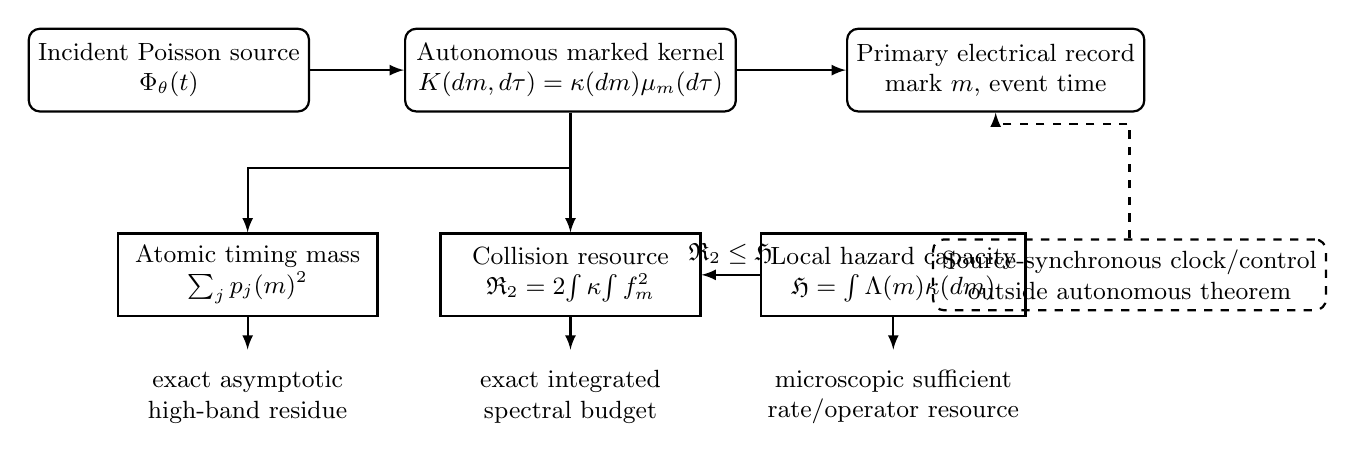
\begin{tikzpicture}[>=latex, line width=0.8pt, font=\small]
  \node[draw, rounded corners, minimum width=3.4cm, minimum height=1.05cm, align=center] (src) at (0,0)
    {Incident Poisson source\\$\Phi_\theta(t)$};
  \node[draw, rounded corners, minimum width=4.2cm, minimum height=1.05cm, align=center] (ker) at (5.1,0)
    {Autonomous marked kernel\\$K(dm,d\tau)=\kappa(dm)\mu_m(d\tau)$};
  \node[draw, rounded corners, minimum width=3.7cm, minimum height=1.05cm, align=center] (rec) at (10.5,0)
    {Primary electrical record\\mark $m$, event time};

  \draw[->] (src) -- (ker);
  \draw[->] (ker) -- (rec);

  \node[draw, minimum width=3.3cm, minimum height=1.05cm, align=center] (atom) at (1.0,-2.6)
    {Atomic timing mass\\$\sum_j p_j(m)^2$};
  \node[draw, minimum width=3.3cm, minimum height=1.05cm, align=center] (r2) at (5.1,-2.6)
    {Collision resource\\$\mathfrak R_2=2\!\int\kappa\!\int f_m^2$};
  \node[draw, minimum width=3.3cm, minimum height=1.05cm, align=center] (haz) at (9.2,-2.6)
    {Local hazard capacity\\$\mathfrak H=\int\Lambda(m)\kappa(dm)$};

  \draw[->] (ker.south) -- ++(0,-0.7) -| (atom.north);
  \draw[->] (ker.south) -- (r2.north);
  \draw[->] (haz.west) -- node[above] {$\mathfrak R_2\le\mathfrak H$} (r2.east);

  \node[align=center] at (1.0,-4.15)
    {exact asymptotic\\high-band residue};
  \node[align=center] at (5.1,-4.15)
    {exact integrated\\spectral budget};
  \node[align=center] at (9.2,-4.15)
    {microscopic sufficient\\rate/operator resource};

  \draw[->] (atom.south) -- (1.0,-3.55);
  \draw[->] (r2.south) -- (5.1,-3.55);
  \draw[->] (haz.south) -- (9.2,-3.55);

  \node[draw, dashed, rounded corners, minimum width=4.0cm, minimum height=0.9cm, align=center] (clock) at (12.2,-2.6)
    {Source-synchronous clock/control\\outside autonomous theorem};
  \draw[dashed,->] (clock.north) -- ++(0,1.45) -| (rec.south);
\end{tikzpicture}
\caption{Resource hierarchy for the autonomous marked-event theorem. The per-photon kernel maps an incident photon into a primary electrical mark and registration delay. Atomic timing mass controls the exact asymptotic flat-band residue; the capture-weighted collision intensity $\mathfrak R_2$ fixes the integrated transfer spectrum; and a capture-weighted local hazard capacity $\mathfrak H$ supplies a microscopic sufficient bound. An external source-synchronous temporal reference is a separate resource and lies outside the autonomous theorem.}
\label{fig:resourceHierarchy}
\end{figure*}


\section{Autonomous marked event channel}

\subsection{Source normalization}

Let the incident photon flux be
\begin{equation}
\Phi_\theta(t)=\Phi_0[1+\theta\cos(\omega t)],\qquad |\theta|\ll1,
\label{eq:source}
\end{equation}
modeled as an inhomogeneous Poisson process. Over long observation times, the incident Fisher-information rate at $\theta=0$ is
\begin{equation}
\dot F_{\rm in}=\frac{\Phi_0}{2}.
\label{eq:inputFI}
\end{equation}
For this paper we normalize every electrical-record Fisher information by Eq.~\eqref{eq:inputFI}. The source model is intentionally classical/direct-detection specific; no claim is made here for arbitrary optical phase encodings or nonclassical input states.

\subsection{Marked subprobability kernel}

Let $\M$ be the complete accessible mark space of the \emph{primary} electrical event. Per incident photon, define the autonomous subprobability kernel
\begin{equation}
K(dm,d\tau)=\kappa(dm)\,\mu_m(d\tau),
\label{eq:kernel}
\end{equation}
where $\tau\ge0$ is registration delay relative to photon arrival. The finite measure $\kappa$ has total mass
\begin{equation}
\eta=\kappa(\M)\le1,
\end{equation}
and $\mu_m$ is a normalized conditional delay probability measure for $\kappa$-almost every mark.

Two assumptions are essential. First, $\kappa$ and $\mu_m$ are independent of the small parameter $\theta$: the source parameter modulates arrival intensity, not the per-photon detector channel. Second, translation covariance in time is part of autonomy: the kernel depends on elapsed delay, not on absolute source phase. A source-synchronous reference violates the latter assumption and is treated below.

Define
\begin{equation}
H_m(\omega)=\int_0^\infty e^{-i\omega\tau}\,d\mu_m(\tau).
\end{equation}
Standard Poisson marking and displacement preserve the Poisson property \cite{Kingman1993,DaleyVereJones2003}.

\begin{theorem}[Exact marked-event information transfer]
For Eq.~\eqref{eq:source} and the autonomous one-primary-event kernel Eq.~\eqref{eq:kernel}, the ideal primary marked electrical record has source-normalized Fisher-information transfer
\begin{equation}
\boxed{
G(\omega)=\int_{\M}|H_m(\omega)|^2\,\kappa(dm).}
\label{eq:G}
\end{equation}
Any parameter-independent background addition or stochastic downstream processing satisfies
\begin{equation}
\eta_I^{\rm measured}(\omega)\le G(\omega).
\label{eq:DP}
\end{equation}
\end{theorem}

\begin{proof}
At $\theta=0$, the marked output intensity measure is $\Phi_0\kappa(dm)$. Convolution with the delay law multiplies the sinusoidal intensity derivative in mark $m$ by $H_m(\omega)$. The Fisher-information rate of a Poisson process with intensity measure $\lambda_\theta$ is the integral of $(\partial_\theta\lambda)^2/\lambda$; time averaging contributes the same factor $1/2$ as in Eq.~\eqref{eq:inputFI}. Division by the incident rate gives Eq.~\eqref{eq:G}. Equation~\eqref{eq:DP} is classical Fisher-information data processing.
\end{proof}

At zero frequency, $G(0)=\eta$. The mark is defined to contain every primary-event variable available to the final estimator. Intentionally discarding a mark is downstream coarse graining and can only reduce FI.

\section{Atomic timing and the exact high-band residue}

A delay law need not possess a density. Let $p_j(m)$ be the masses of the atoms of $\mu_m$. Wiener's theorem for Fourier transforms of finite measures \cite{Katznelson2004} gives
\begin{equation}
\lim_{\Omega\to\infty}\frac{1}{2\Omega}
\int_{-\Omega}^{\Omega}|H_m(\omega)|^2d\omega
=\sum_jp_j(m)^2.
\end{equation}
Because $|H_m|\le1$ and $\kappa$ is finite, dominated convergence gives the marked result.

\begin{theorem}[Atomic timing residue]
\begin{equation}
\boxed{
\lim_{\Omega\to\infty}\frac{1}{2\Omega}
\int_{-\Omega}^{\Omega}G(\omega)d\omega
=\int_{\M}\left[\sum_jp_j(m)^2\right]\kappa(dm).}
\label{eq:atomic}
\end{equation}
\end{theorem}

Thus purely non-atomic mark-conditioned delay laws force the flat-band average information transfer to vanish asymptotically. This statement is about the band average; it does not assert pointwise decay for every singular continuous probability measure. Deterministic or discrete timing branches leave an exact residue. A very narrow continuous prompt component has zero ultimate Wiener residue but can move the crossover to arbitrarily high frequency; a quantitative resource is therefore still needed.

\section{Timing-collision spectral resource}

Assume now that every $\mu_m$ has a square-integrable density $f_m(t)$. Define
\begin{equation}
\boxed{
\Rtwo=2\int_{\M}\kappa(dm)\int_0^\infty f_m(t)^2dt.}
\label{eq:R2}
\end{equation}
This capture-weighted timing-collision intensity has dimensions of inverse time.

\begin{theorem}[Exact timing-spectrum sum rule]
Parseval's identity gives
\begin{equation}
\boxed{
\int_{-\infty}^{\infty}G(\omega)d\omega=\pi\Rtwo.}
\label{eq:parseval}
\end{equation}
Consequently,
\begin{equation}
\boxed{
\bar\eta_I(\Omega)
\equiv\frac{1}{2\Omega}\int_{-\Omega}^{\Omega}G(\omega)d\omega
\le\min\left[\eta,\frac{\pi\Rtwo}{2\Omega}\right].}
\label{eq:flat}
\end{equation}
\end{theorem}

A target average transfer $q$ therefore requires $q\le\eta$ and
\begin{equation}
\Omega\le\frac{\pi\Rtwo}{2q},
\qquad
B\equiv\frac{\Omega}{2\pi}\le\frac{\Rtwo}{4q}.
\end{equation}
Here $B$ is an information-task half-band in ordinary frequency, not an electrical $-3\,$dB bandwidth.

\subsection{Weighted spectral tasks}

Let $w(\omega)\ge0$ be a normalized weighting of frequency-resolved source-FI tasks,
\begin{equation}
\int_{-\infty}^{\infty}w(\omega)d\omega=1,
\end{equation}
and define
\begin{equation}
\Wcal(A)=\sup_{E:\,|E|\le A}\int_Ew(\omega)d\omega,
\label{eq:W}
\end{equation}
where the supremum is over measurable frequency sets of Lebesgue measure at most $A$. Since $0\le G\le\eta$ and Eq.~\eqref{eq:parseval} fixes its $L^1$ spectral budget, the bathtub/rearrangement principle gives
\begin{equation}
\boxed{
\int w(\omega)G(\omega)d\omega
\le\eta\,\Wcal\!\left(\frac{\pi\Rtwo}{\eta}\right),\qquad \eta>0.}
\label{eq:arbsource}
\end{equation}
Equation~\eqref{eq:flat} is recovered for uniform $w$ on $[-\Omega,\Omega]$. Equation~\eqref{eq:arbsource} is not asserted to cover arbitrary correlated multiparameter estimation across frequency.

\section{Microscopic completion by local registration intensity}

For an absolutely continuous conditional delay law define survival $S_m(t)$ and hazard
\begin{equation}
h_m(t)=\frac{f_m(t)}{S_m(t)}.
\end{equation}
Suppose $h_m(t)\le\Lambda(m)$ almost everywhere and define the capture-weighted hazard capacity
\begin{equation}
\boxed{\Hcap=\int_{\M}\Lambda(m)\kappa(dm).}
\label{eq:Hcap}
\end{equation}

\begin{lemma}[Hazard--collision inequality]
\begin{equation}
\boxed{\Rtwo\le\Hcap.}
\label{eq:R2H}
\end{equation}
\end{lemma}

\begin{proof}
For a normalized continuous delay law, $S_m(0)=1$ and $S_m(t)\to0$. Since $f_m=h_mS_m$,
\begin{equation}
\int_0^\infty f_m^2dt
=\int_0^\infty h_m^2S_m^2dt
\le\Lambda(m)\int_0^\infty h_mS_m^2dt.
\end{equation}
But $dS_m^2/dt=-2h_mS_m^2$, so
\begin{equation}
\int_0^\infty h_mS_m^2dt=\frac12.
\end{equation}
Therefore $2\int f_m^2dt\le\Lambda(m)$. Integrating over $\kappa(dm)$ proves Eq.~\eqref{eq:R2H}.
\end{proof}

Thus
\begin{equation}
\boxed{
\bar\eta_I(\Omega)
\le\min\left[\eta,\frac{\pi\Hcap}{2\Omega}\right].}
\label{eq:Hbound}
\end{equation}
A uniform hazard ceiling $\Lambda(m)\le\Lambda$ implies
\begin{equation}
\bar\eta_I(\Omega)\le
\eta\min\left[1,\frac{\pi\Lambda}{2\Omega}\right].
\label{eq:uniformH}
\end{equation}
The weighted form is strictly sharper: an arbitrarily fast branch does not matter if its capture weight becomes correspondingly negligible.

\begin{corollary}[Minimum timing-resource cost]
For a flat source-information task on $|\omega|\le\Omega$, let
\begin{equation}
B\equiv\frac{\Omega}{2\pi}
\end{equation}
be the ordinary-frequency half-band. Achieving absolute average transfer
\begin{equation}
\bar\eta_I(\Omega)\ge q>0
\end{equation}
requires $q\le\eta$ and
\begin{equation}
\boxed{\Rtwo\ge4Bq,\qquad \Hcap\ge4Bq.}
\label{eq:resourceCost}
\end{equation}
If the markwise hazards share a uniform ceiling $\Lambda(m)\le\Lambda$, then $\Hcap\le\eta\Lambda$ and therefore
\begin{equation}
\boxed{\Lambda\ge\frac{4Bq}{\eta}.}
\label{eq:uniformResourceCost}
\end{equation}
For a target retention $q=r\eta$ relative to the captured DC information, this reduces to $\Lambda\ge4Br$.
\end{corollary}

For constant hazard $f(t)=\Lambda e^{-\Lambda t}$,
\begin{equation}
H(\omega)=\frac{\Lambda}{\Lambda+i\omega},
\end{equation}
and
\begin{equation}
\frac{1}{2\Omega}\int_{-\Omega}^{\Omega}|H(\omega)|^2d\omega
=\frac{\Lambda}{\Omega}\tan^{-1}\!\left(\frac{\Omega}{\Lambda}\right)
\sim\frac{\pi\Lambda}{2\Omega}.
\end{equation}
Hence the high-band coefficient in Eq.~\eqref{eq:uniformH} is asymptotically tight.

For a classical Markov detector, a sufficient uniform $\Lambda$ is the maximum total intensity of all first-registration transitions from any pre-registration state. For quantum-jump registration, a sufficient bound is $\|\sum_\alpha L_\alpha^\dagger L_\alpha\|_\infty$. These are local rate/operator resources, not stationary activities.

\section{Exactly fixed mean and RMS jitter do not bound information bandwidth}

Fix target mean $\mu_0>0$ and variance $\sigma^2>0$. Consider
\begin{equation}
f_{\epsilon,n,\lambda}(t)
=(1-\epsilon)ne^{-nt}
+\epsilon\lambda e^{-\lambda t},
\qquad 0<\epsilon<1.
\end{equation}
Write $x=1/\lambda$. The variance is
\begin{equation}
V_{\epsilon,n}(x)
=\frac{2(1-\epsilon)}{n^2}+2\epsilon x^2
-\left[\frac{1-\epsilon}{n}+\epsilon x\right]^2.
\end{equation}
For sufficiently large $n$, the equation $V_{\epsilon,n}(x)=\sigma^2$ has the positive solution
\begin{equation}
\boxed{
x_{\epsilon,n}
=\frac{
\sqrt{(2-\epsilon)n^2\sigma^2-2(1-\epsilon)}
+\sqrt\epsilon(1-\epsilon)
}{
\sqrt\epsilon\,n(2-\epsilon)
}.}
\label{eq:exactx}
\end{equation}
Set $\lambda_{\epsilon,n}=1/x_{\epsilon,n}$. Then
\begin{equation}
\operatorname{Var}(X_{\epsilon,n})=\sigma^2
\end{equation}
exactly. Moreover,
\begin{equation}
\mathbb E X_{\epsilon,n}\to
\sigma\sqrt{\frac{\epsilon}{2-\epsilon}}
\end{equation}
as $n\to\infty$, and this limit tends to zero with $\epsilon$.

Choose $\epsilon$ sufficiently small and $n$ sufficiently large that $\mathbb E X_{\epsilon,n}<\mu_0$, and define
\begin{equation}
D_{\epsilon,n}=X_{\epsilon,n}
+\mu_0-\mathbb E X_{\epsilon,n}.
\end{equation}
Then every chosen family member satisfies
\begin{equation}
\boxed{
\mathbb E D_{\epsilon,n}=\mu_0,
\qquad
\operatorname{Var}(D_{\epsilon,n})=\sigma^2.}
\end{equation}
The deterministic shift changes only the phase of the characteristic function. For the unshifted mixture,
\begin{equation}
H_{\epsilon,n}(\omega)
=(1-\epsilon)\frac{n}{n+i\omega}
+\epsilon\frac{\lambda_{\epsilon,n}}{\lambda_{\epsilon,n}+i\omega}.
\end{equation}
For every prescribed finite band $|\omega|\le\Omega_*$,
\begin{equation}
\limsup_{n\to\infty}
\sup_{|\omega|\le\Omega_*}
|H_{\epsilon,n}(\omega)-1|
\le2\epsilon.
\end{equation}
Taking $\epsilon\to0$ gives $|H_{D_{\epsilon,n}}(\omega)|^2\to1$ uniformly on the band. Therefore
\begin{equation}
\boxed{
\{\mathbb E D=\mu_0,\operatorname{Var}D=\sigma^2\}
\not\Rightarrow
\text{finite temporal information bandwidth}.}
\end{equation}
This does not say that a complete specified IRF is irrelevant. It rejects low-order moments as architecture-independent timing resources. Likewise, an FWHM or other scalar width is not a complete substitute for the timing law without additional shape assumptions.

\begin{figure}[t]
\centering
\begin{tikzpicture}
\begin{loglogaxis}[
  width=0.95\columnwidth,
  height=0.68\columnwidth,
  xmin=1e-2,xmax=2e4,
  ymin=1e-4,ymax=1.05,
  xlabel={$\omega\sigma$},
  ylabel={$|H(\omega)|^2$},
  grid=major,
  legend style={font=\scriptsize,at={(0.03,0.05)},anchor=south west,draw=none,fill=none},
  tick label style={font=\scriptsize},
  label style={font=\small},
]
\addplot+[very thick] table[x=omega_sigma,y=eps020_n50,col sep=comma] {fig_jitter_no_go_data.csv};
\addlegendentry{$\epsilon=0.20,\ n\sigma=50$}
\addplot+[very thick,dashed] table[x=omega_sigma,y=eps005_n200,col sep=comma] {fig_jitter_no_go_data.csv};
\addlegendentry{$\epsilon=0.05,\ n\sigma=200$}
\addplot+[very thick,dashdotted] table[x=omega_sigma,y=eps001_n1000,col sep=comma] {fig_jitter_no_go_data.csv};
\addlegendentry{$\epsilon=0.01,\ n\sigma=1000$}
\addplot[thin,dotted,domain=1e-2:2e4] {0.5};
\end{loglogaxis}
\end{tikzpicture}
\caption{Exact low-order-jitter no-go. Each curve belongs to the WP33 two-path family after a deterministic shift chosen so that every detector has the same prescribed mean $\mu_0=2\sigma$ and the same exact variance $\sigma^2$. Decreasing the rare-path probability $\epsilon$ while increasing the fast-path rate $n$ pushes substantial information transfer to progressively larger $\omega\sigma$, despite identical mean delay and RMS jitter. The plotted deterministic shift affects only Fourier phase and therefore does not change $|H|^2$.}
\label{fig:jitterNoGo}
\end{figure}


\section{External temporal reference is an independent resource}
\label{sec:clock}

Autonomy cannot be dropped for free. Suppose a detector possesses a phase-locked clock at the modulation frequency and stores at photon arrival the phase mark
\begin{equation}
M=\omega t\pmod{2\pi}.
\end{equation}
Equation~\eqref{eq:source} then induces
\begin{equation}
p_\theta(M)=\frac{1}{2\pi}[1+\theta\cos M].
\end{equation}
At $\theta=0$ the mark carries FI $1/2$ per captured photon, equal to the incident timing FI per photon. It may be reported after an arbitrarily slow final registration without losing the stored phase information.

Thus detector-only timing bounds can be defeated by a free source-synchronous reference. A theorem for heterodyne, gated, lock-in, or other clocked architectures must count temporal-reference frequency, phase precision, control action, memory, or an equivalent resource. The present theorem instead assumes autonomous/time-translation-invariant processing.

\section{Thermodynamic no-go and conditional repair}
\label{sec:thermo}

Consider a restricted reversible \emph{finite-state, time-homogeneous continuous-time Markov} optical gateway
\begin{equation}
0\xrightleftharpoons[d]{u}1,
\end{equation}
with stationary forward optical traffic $f=u\pi_0$ and reverse traffic $r=d\pi_1$. Assume $f\ge r$, useful throughput $f\ge f_*>0$, total dimensionless entropy-production rate $\sigma_{\rm tot}\le\Sigma$, and stationary one-way activity $\mathcal A_{\rm tot}\le\mathcal A$.

Set $z=f/r\ge1$ and
\begin{equation}
g(z)=\left(1-\frac1z\right)\ln z,
\qquad
Z_*=g^{-1}(\Sigma/f_*).
\end{equation}
Since the optical-edge entropy production is $f g(z)$,
\begin{equation}
\pi_1=\frac{f}{dz}\ge\frac{f_*}{dZ_*}.
\end{equation}
If $\lambda_1$ is the total first-exit rate from state 1, activity gives
\begin{equation}
\boxed{
\lambda_1\le\Lambda_*
\equiv\frac{\mathcal A d}{f_*}
 g^{-1}\!\left(\frac{\Sigma}{f_*}\right).}
\label{eq:Lstar}
\end{equation}

Suppose no primary electrical registration can occur before the first exit from state 1. In a time-homogeneous finite-state continuous-time Markov chain, the holding time $T_1\sim\mathrm{Exp}(\lambda_1)$ is independent of exit destination. We additionally restrict the accessible downstream mark $M$ to be generated from the exit destination and subsequent autonomous Markov path, so the memoryless downstream dynamics does not retain the realized gateway holding time. Hence
\begin{equation}
D\mid M=T_1+Y_M,
\qquad Y_M\ge0,
\end{equation}
with $T_1$ independent of $(M,Y_M)$. Then
\begin{align}
f_D(t\mid M)&=\lambda_1\int_0^t e^{-\lambda_1(t-y)}dF_{Y_M}(y),\\
S_D(t\mid M)&=\Pr(Y_M>t\mid M)+\int_0^t e^{-\lambda_1(t-y)}dF_{Y_M}(y),
\end{align}
which implies
\begin{equation}
\boxed{h_D(t\mid M)\le\lambda_1\le\Lambda_*.}
\label{eq:bridge}
\end{equation}
Therefore
\begin{equation}
\boxed{
\bar\eta_I(\Omega)
\le C\min\left[
1,
\frac{\pi\mathcal A d}{2f_*\Omega}
 g^{-1}\!\left(\frac{\Sigma}{f_*}\right)
\right],}
\label{eq:thermo}
\end{equation}
where $C$ is any upper bound on primary-event probability. The explicit exponential gateway also yields the stronger pointwise envelope
\begin{equation}
\eta_I(\omega)\le
C\frac{\Lambda_*^2}{\Lambda_*^2+\omega^2}.
\end{equation}

The absolute reverse optical rate $d$ in Eq.~\eqref{eq:Lstar} is a microscopic rate resource. It cannot in general be removed in favor of stationary aggregate thermodynamic quantities. Appendix~\ref{app:rare-fast} gives a reversible three-state family with fixed optical forward/reverse rate ratio, finite useful optical traffic, bounded stationary activity, and bounded total steady entropy production, while its post-capture local rate and information bandwidth diverge. The construction does not keep every nonoptical bare affinity fixed; its purpose is precisely to show that the stated aggregate thermodynamic resources do not control all hidden microscopic scales. Thus
\begin{equation}
\boxed{
\text{stationary aggregate thermodynamic budgets alone do not determine the temporal information scale}.}
\end{equation}
For a weakly coupled thermal bosonic optical reservoir one may have $d=\gamma(\omega_0)[n_T(\omega_0)+1]$; temperature only supplies a speed statement after the absolute coupling spectrum $\gamma(\omega_0)$ is separately bounded.

\section{Relation to detector metrics and prior work}

A deterministic transit time is latency; unresolved transit dispersion can reduce information. An RC pole is an amplitude bandwidth and becomes an information limit only after the observation/noise model makes filtered degrees of freedom irrecoverable. Low-order timing moments do not control prompt concentration. The resources in Eqs.~\eqref{eq:atomic}, \eqref{eq:R2}, and \eqref{eq:Hcap} target these distinct questions.

Talaga's TCSPC analysis already emphasized IRF-induced information loss, detector sensitivity--bandwidth tradeoffs, and the frequency-domain power spectrum of detector IRFs \cite{Talaga2009}. K\"ollner and Wolfrum quantified photon requirements for lifetime estimation \cite{KollnerWolfrum1992}; later FI analyses explicitly included finite IRFs and photon statistics \cite{Bouchet2019,TrinhEsposito2021}. Our parameter is instead a modulation of the incident source itself, and our claims concern the exact marked-event transfer theorem plus the atomic/collision/hazard resource hierarchy and its no-go/repair statements.

Recent finite-frequency fluctuation--response inequalities bound response precision by dynamical activity or related resources in Markov systems \cite{Dechant2026}. Those results are pointwise response/noise inequalities and use different broadband quantities. Equation~\eqref{eq:parseval} instead follows from the first-registration timing measure. We do not claim generic finite-frequency response--noise inequalities as new.

\section{Scope and limitations}

The independent-event kernel assumes a low-overlap regime. History-dependent capture, saturation, and recovery require a trajectory-level extension. A dead-time or threshold map applied after a sufficient latent primary record cannot increase FI, but history-dependent capture is outside Eq.~\eqref{eq:kernel}.

Multiple offspring after a sufficient primary event are downstream processing. Multiple independent \emph{pre-primary} timing records generated from one absorbed photon constitute an additional multiplicity resource and are outside the one-primary-event class.

The source is weak coherent/direct-detection intensity modulation. Nonclassical statistics and phase-sensitive source parameters require a separate input-information treatment.

The thermodynamic mark bridge uses finite-state Markov memorylessness. Semi-Markov or age-dependent detectors that explicitly retain gateway dwell time require an enlarged state/control resource and are not covered by Eq.~\eqref{eq:bridge} without further analysis.

Finally, Eq.~\eqref{eq:thermo} is a restricted thermodynamic completion, not a universal temperature law. Material-specific predictions require microscopic relations from temperature and device resources to capture, unavoidable background, and absolute local transition intensities.

\section{Discussion and conclusion}

For autonomous event detection, temporal information resources form a hierarchy. Atomic timing mass determines the exact asymptotic high-band residue. The capture-weighted collision intensity $\Rtwo$ fixes the integrated source-information transfer spectrum. The capture-weighted local hazard capacity $\Hcap$ is a microscopic sufficient resource satisfying $\Rtwo\le\Hcap$. Equivalently, preserving absolute average information fraction $q$ over ordinary-frequency half-band $B$ requires the minimum cost $\Hcap\ge4Bq$. Stationary activity and entropy production do not generally control these local timing resources because arbitrarily fast dynamics can hide in rarely occupied states; a restricted thermodynamic repair appears only after an absolute microscopic rate is supplied.

The result also clarifies why different photodetector classes require different resources. An actively synchronized detector possesses a temporal reference. A coherent pointer can store information before any registered event. Continuous analog detection may be better described by response/noise or channel-capacity bounds. The present theorem is therefore one closed branch of a broader photodetection resource theory, not a scalar speed law for every architecture.

\appendix
\input{appendix_rare_fast_counterexample}

\bibliography{references}
\end{document}
